% 2009 年福建卷理科第 17 题：正方形 ABCD 与两条垂线 MD、NB。
% 来源 PDF：普通高考/2009/2009福建理.pdf，SHA-256 44d650687de50fff3efc1d37624b1272c9045e96d41491464f6713a708f202b9。
% 原页：第 1 页（A3 三栏）第 3 栏上部，书页码 515。
% 重绘依据：正方形边长 1，MD=NB=1，E 为 BC 中点；斜二测投影。
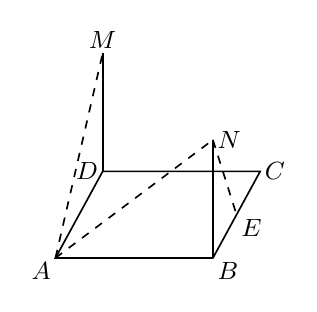
\begin{tikzpicture}[semithick, every node/.style={inner sep=1.4pt, font=\small}]
  \coordinate (A) at (0.0,0.0);
  \coordinate (B) at (2.0,0.0);
  \coordinate (C) at (2.6,1.1);
  \coordinate (D) at (0.6,1.1);
  \coordinate (M) at (0.6,2.6);
  \coordinate (N) at (2.0,1.5);
  \coordinate (E) at (2.3,0.55);
  % 底面
  \draw (A) -- (B) -- (C) -- (D) -- cycle;
  % 垂线
  \draw (M) -- (D);
  \draw (N) -- (B);
  % 辅助线
  \draw[dashed] (A) -- (M);
  \draw[dashed] (A) -- (N);
  \draw[dashed] (N) -- (E);
  % 标注
  \node[below left] at (A) {$A$};
  \node[below right] at (B) {$B$};
  \node[right] at (C) {$C$};
  \node[left] at (D) {$D$};
  \node[above] at (M) {$M$};
  \node[right] at (N) {$N$};
  \node[below right] at (E) {$E$};
\end{tikzpicture}
